\documentclass{article}

\usepackage{amsmath,amssymb}
\usepackage{geometry}
\usepackage{graphicx}

\geometry{a4paper, margin=2.5cm}

\begin{document}

% ============================================================
\section*{Markov Decision Processes (MDP)}

\subsection*{First, a story}

Imagine you are a mouse living in a $3\times 3$ maze. Each move goes up, down, left, or right. Reaching the cheese cell gives $+1$, the shock cell gives $-1$, everything else scores nothing. Your goal: find a route that maximizes the long-run total score.

This story is an MDP. Let us translate its ingredients into mathematics.

\subsection*{Formalization: the five-tuple}

An MDP is fully described by five elements:

\[
\boxed{\mathcal{M} = (\mathcal{S}, \mathcal{A}, \mathcal{P}, \mathcal{R}, \gamma)}
\]

\begin{itemize}
  \item $\mathcal{S}$ --- the \textbf{state space} (in the maze, $\mathcal{S}=\{1,\ldots,9\}$);
  \item $\mathcal{A}$ --- the \textbf{action space} ($\mathcal{A}=\{\uparrow,\downarrow,\leftarrow,\rightarrow\}$, $|\mathcal{A}|=4$);
  \item $\mathcal{P}$ --- the \textbf{transition probabilities}. The Markov property: the next state depends only on the current state and action, not on earlier history:
        \[
        P(S_{t+1}=s' \mid S_t=s, A_t=a, S_{t-1}, A_{t-1},\ldots,S_0) = P(S_{t+1}=s' \mid S_t=s, A_t=a)
        \]
        abbreviated $P^{a}_{ss'} = P(s'\mid s,a)$. For every $s,a$ it forms a distribution: $\sum_{s'\in\mathcal{S}}P(s'\mid s,a)=1$;
  \item $\mathcal{R}$ --- the \textbf{reward function}. $R(s,a)=\mathbb{E}[R_{t+1}\mid S_t=s, A_t=a]$ is the expected immediate reward (it may also be written $R(s,a,s')$);
  \item $\gamma \in [0,1)$ --- the \textbf{discount factor}. $\gamma\to 0$ is myopic, $\gamma\to 1$ far-sighted; $\gamma<1$ guarantees convergence of the infinite-horizon return series (given bounded rewards).
\end{itemize}

\subsection*{The interaction loop}

Agent and environment interact at discrete steps $t=0,1,2,\ldots$, each producing a tuple $(S_t, A_t, R_{t+1}, S_{t+1})$; the full trajectory is:

\[
S_0, A_0, R_1, S_1, A_1, R_2, S_2, \ldots
\]

Its joint distribution is determined by $\mathcal{P}$ and the policy $\pi$ --- the source of all data in reinforcement learning: try, observe feedback, adjust, repeat.

% ============================================================
\section*{Value Functions --- What Makes a State ``Good''}

\subsection*{Return}

One cannot judge a single step in isolation --- the cheese may be next door or ten cells away. Define the \textbf{discounted return}:

\[
\boxed{G_t = R_{t+1} + \gamma R_{t+2} + \gamma^2 R_{t+3} + \cdots = \sum_{k=0}^{\infty} \gamma^k R_{t+k+1}}
\]

Summing all future rewards with heavier discounting the further out they are. Its recursive form is the starting point of every Bellman derivation:

\[
\boxed{G_t = R_{t+1} + \gamma G_{t+1}}
\]

\subsection*{Value functions: conditional expectations of the return}

Because transitions are stochastic you cannot predict the future exactly; take expectations:

\[
\boxed{v_\pi(s) = \mathbb{E}_\pi[G_t \mid S_t = s]}, \qquad
\boxed{q_\pi(s,a) = \mathbb{E}_\pi[G_t \mid S_t = s, A_t = a]}
\]

\begin{itemize}
  \item $v_\pi(s)$ --- starting from state $s$ under policy $\pi$, the expected return (\textbf{state value});
  \item $q_\pi(s,a)$ --- taking action $a$ first in state $s$, then following $\pi$ (\textbf{action value}).
\end{itemize}

In one sentence: value is not the exact future, but the conditional expectation of the return.

\subsection*{Relations between $v_\pi$ and $q_\pi$}

From the definitions, each recovers the other:

\[
v_\pi(s) = \sum_{a\in\mathcal{A}} \pi(a\mid s)\, q_\pi(s,a)
\]
\[
q_\pi(s,a) = R(s,a) + \gamma \sum_{s'\in\mathcal{S}} P(s'\mid s,a)\, v_\pi(s')
\]

State value = the policy-weighted average of action values; action value = immediate reward + discounted expected successor value. Both relations recur throughout the Bellman derivations.

% ============================================================
\section*{The Bellman Expectation Equation --- Splitting the Future into ``Now + Later''}

\subsection*{Derivation}

Bellman's key insight: value can be defined \textbf{recursively}. Starting from $G_t = R_{t+1} + \gamma G_{t+1}$:

\[
\begin{aligned}
v_\pi(s) &= \mathbb{E}_\pi[G_t \mid S_t=s] \\
&= \mathbb{E}_\pi[R_{t+1} + \gamma G_{t+1} \mid S_t=s] \\
&= \mathbb{E}_\pi[R_{t+1}\mid S_t=s] + \gamma\,\mathbb{E}_\pi[G_{t+1}\mid S_t=s]
\end{aligned}
\]

The first term is the expected immediate reward; the second is the expected successor value. Expanding over actions $a$ and successor states $s'$:

\[
\boxed{v_\pi(s) = \sum_{a\in\mathcal{A}} \pi(a\mid s) \left[ R(s,a) + \gamma \sum_{s'\in\mathcal{S}} P(s'\mid s,a)\, v_\pi(s') \right]}
\]

You never need to look infinitely far ahead: look one step, then use the next state's value. The action-value form is analogous:

\[
q_\pi(s,a) = R(s,a) + \gamma \sum_{s'\in\mathcal{S}} P(s'\mid s,a) \sum_{a'\in\mathcal{A}} \pi(a'\mid s')\, q_\pi(s',a')
\]

\subsection*{A concrete example}

Suppose you are in cell A, moving right deterministically lands in cell B, with reward $R=0$. If $v(B)=5$ and $\gamma=0.9$:

\[
q(A, \rightarrow) = 0 + 0.9 \times 5 = 4.5
\]

Cell A itself pays nothing, but sitting next to a ``good place'' makes A good too. That is the recursive power of the Bellman equation --- value propagates across states.

\subsection*{Matrix form (finite MDPs)}

With a finite state space the Bellman expectation equation is a linear system:

\[
\boxed{v_\pi = R_\pi + \gamma P_\pi v_\pi}
\]

with $v_\pi\in\mathbb{R}^{|\mathcal{S}|}$, $R_\pi(s)=\sum_a \pi(a\mid s)R(s,a)$ and $P_\pi(s,s')=\sum_a \pi(a\mid s)P(s'\mid s,a)$. It has the closed-form solution:

\[
v_\pi = (I - \gamma P_\pi)^{-1} R_\pi
\]

This is the only place a closed form exists --- the optimality equation is not so lucky.

% ============================================================
\section*{The Bellman Optimality Equation --- Choosing the Best at Every Step}

\subsection*{Optimal value functions}

Define the optimal value functions as the maximum over all policies:

\[
v_*(s) = \max_\pi v_\pi(s),\quad \forall s\in\mathcal{S}, \qquad
q_*(s,a) = \max_\pi q_\pi(s,a),\quad \forall s\in\mathcal{S},\, a\in\mathcal{A}
\]

For finite MDPs an optimal policy $\pi_*$ always exists with $v_{\pi_*}=v_*$ (state by state); moreover $v_*(s)=\max_a q_*(s,a)$.

\subsection*{Deriving the optimality equation for $v_*$}

Replace the policy-weighted average in the expectation equation by a maximum:

\[
\boxed{v_*(s) = \max_{a\in\mathcal{A}} \left[ R(s,a) + \gamma \sum_{s'\in\mathcal{S}} P(s'\mid s,a)\, v_*(s') \right]}
\]

More rigorously: let $\pi_*$ be optimal, so $v_{\pi_*}=v_*$ and $q_{\pi_*}=q_*$. Substituting $v_* = v_{\pi_*}$ into the action-value expectation equation gives $q_*(s,a) = R(s,a) + \gamma\sum_{s'}P(s'\mid s,a)\,v_*(s')$; maximizing over $a$ via $v_* = \max_a q_*$:

\[
v_*(s) = \max_a q_*(s,a) = \max_a \left[ R(s,a) + \gamma \sum_{s'\in\mathcal{S}} P(s'\mid s,a)\, v_*(s') \right]
\]

The only difference from the expectation equation: $\sum_a \pi(a\mid s)$ becomes $\max_a$. The action-value form:

\[
q_*(s,a) = R(s,a) + \gamma \sum_{s'\in\mathcal{S}} P(s'\mid s,a) \max_{a'\in\mathcal{A}} q_*(s',a')
\]

\subsection*{Why no closed form?}

The expectation equation is linear (invertible); the optimality equation is \textbf{nonlinear} --- the $\max$ operator breaks the linear structure, so no matrix inverse solves it. One can only iterate:

\[
\begin{aligned}
&v_\pi = R_\pi + \gamma P_\pi v_\pi \;\Longrightarrow\; v_\pi = (I-\gamma P_\pi)^{-1}R_\pi \qquad \text{(linear, invertible)}\\
&v_* = \max_a \left(R_a + \gamma P_a v_*\right) \qquad \text{(nonlinear, contains $\max$, not invertible)}
\end{aligned}
\]

That is why dynamic programming (value iteration, policy iteration) exists.

% ============================================================
\section*{From Equations to Algorithms: Policy Improvement and Dynamic Programming}

\subsection*{The policy improvement theorem}

Given any policy $\pi$ and its $q_\pi$, construct $\pi'(s) = \arg\max_a q_\pi(s,a)$; then $\pi'$ is \textbf{no worse} than $\pi$ (i.e., $v_{\pi'} \ge v_\pi$ componentwise) --- the \textbf{policy improvement theorem}. Alternating ``evaluate $\to$ improve'' to a fixed point converges to an optimal policy $\pi_*$.

\subsection*{The three workhorses of dynamic programming}

With a known model $\mathcal{P}$, $\mathcal{R}$, the MDP can be solved exactly. The three algorithms, on a $4\times 4$ GridWorld (goal in the bottom-right corner, entering it gives $+1$, $\gamma=0.9$):

\textbf{Policy evaluation}: iterate the Bellman expectation equation $V_{k+1}(s) \leftarrow \sum_a \pi(a\mid s)\bigl[R(s,a)+\gamma\sum_{s'}P(s'\mid s,a)V_k(s')\bigr]$, converging to $v_\pi$. Figure~\ref{fig:policy-eval} shows several states' $V_k(s)$ converging with sweeps (left) and the converged $v_\pi$ heatmap (right).

\begin{figure}[!htbp]
  \centering
  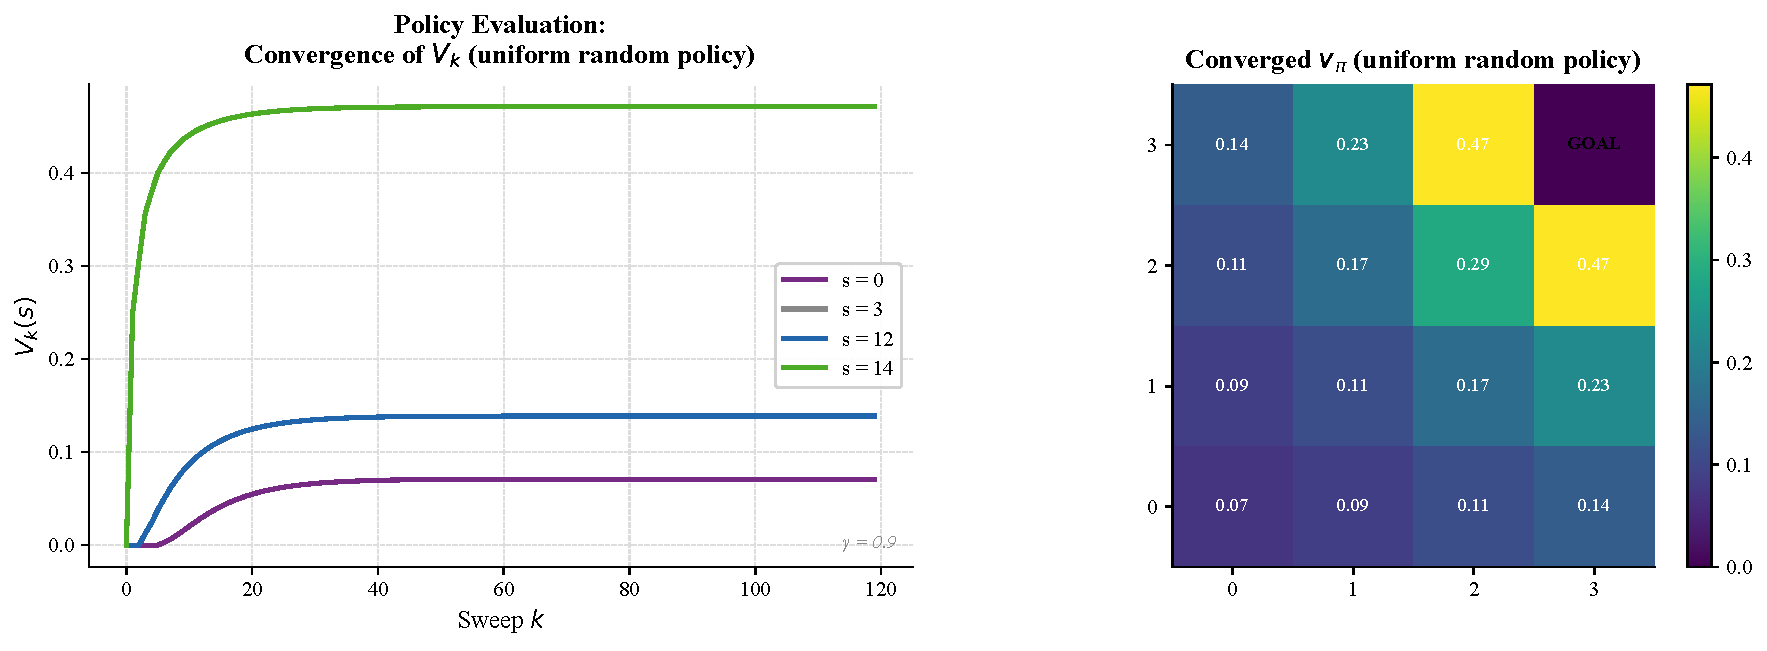
\includegraphics[width=0.85\textwidth]{fig1_policy_evaluation.pdf}
  \caption{Policy evaluation ($4\times4$ GridWorld, uniform random policy, $\gamma=0.9$). Left: $V_k(s)$ of four states converging over sweeps (cells next to the goal converge fast, far corners slowly); right: the converged $v_\pi$ as a heatmap.}
  \label{fig:policy-eval}
\end{figure}

\textbf{Value iteration}: iterate the Bellman optimality equation $V_{k+1}(s) \leftarrow \max_a\bigl[R(s,a)+\gamma\sum_{s'}P(s'\mid s,a)V_k(s')\bigr]$. Figure~\ref{fig:vi-wave} shows high-value regions spreading outward from the goal like a wave.

\begin{figure}[!htbp]
  \centering
  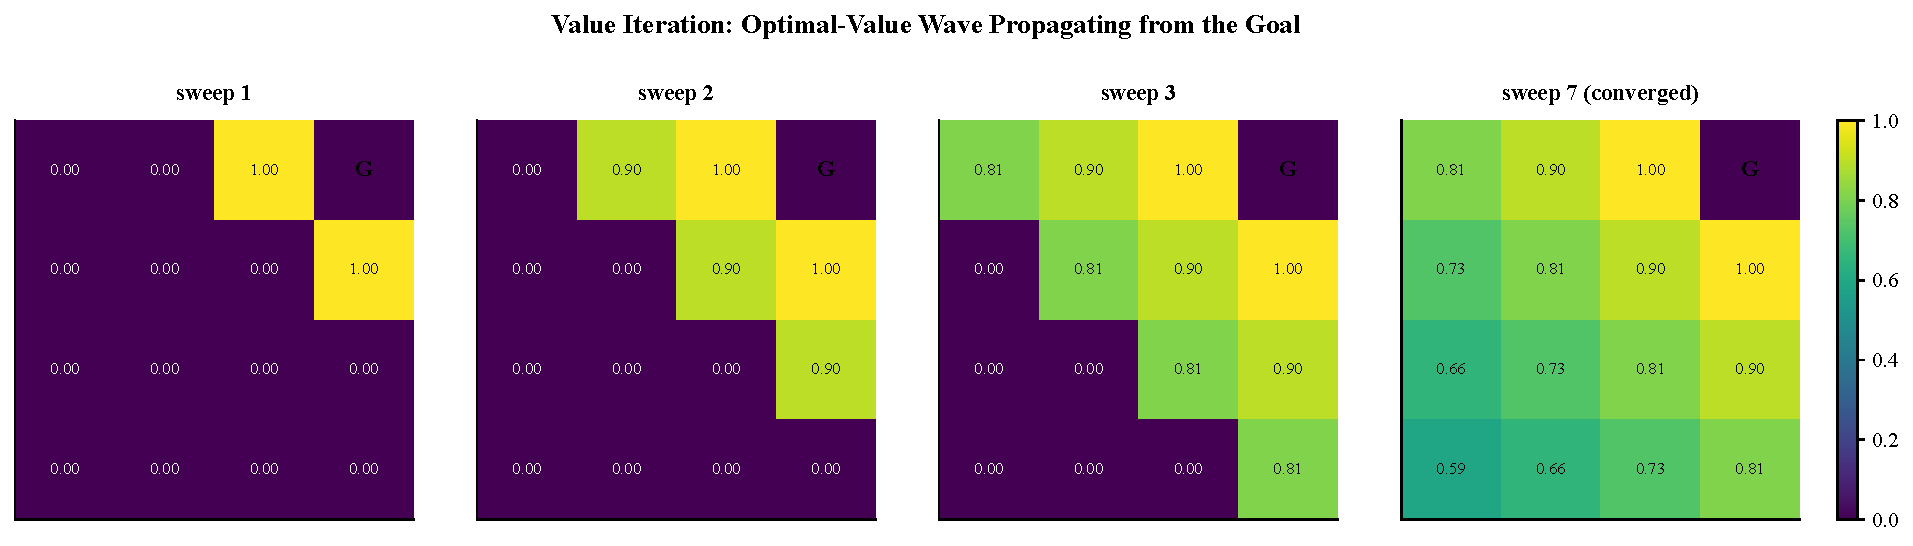
\includegraphics[width=0.85\textwidth]{fig2_value_iteration_wave.pdf}
  \caption{Value propagation under value iteration ($4\times4$ GridWorld, $\gamma=0.9$). $V_k$ at sweeps 1/2/3 and at convergence (sweep 7): cells one step from the goal reach $1.0$ first; each further sweep radiates value one more cell outward.}
  \label{fig:vi-wave}
\end{figure}

\textbf{Policy iteration}: alternate ``full policy evaluation $\to$ greedy improvement''. Figure~\ref{fig:pi-vi} compares the two convergence dynamics.

\begin{figure}[!htbp]
  \centering
  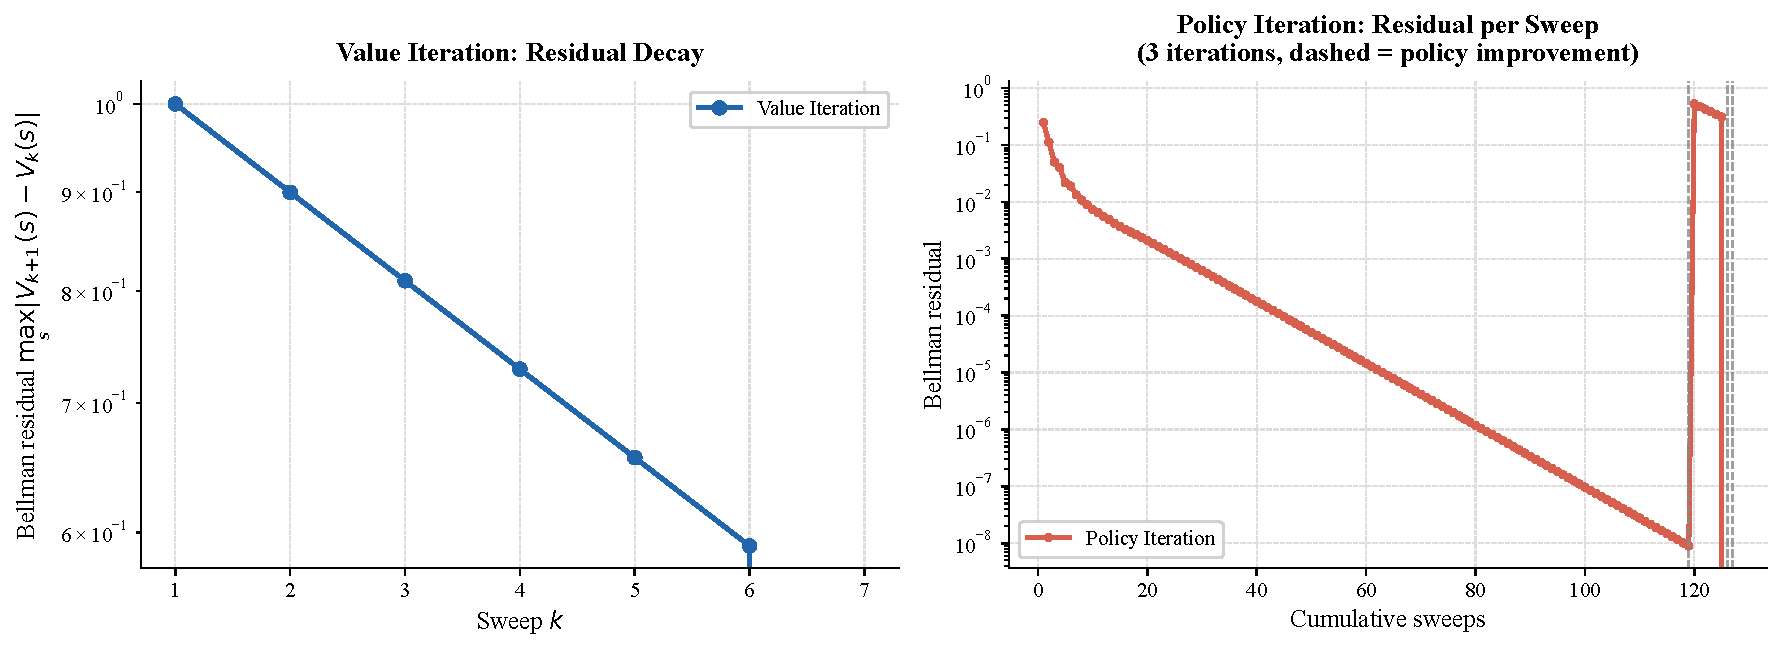
\includegraphics[width=0.88\textwidth]{fig3_policy_vs_value_iteration.pdf}
  \caption{Value iteration vs policy iteration ($4\times4$ GridWorld, $\gamma=0.9$). Left: the Bellman residual $\max_s|V_{k+1}-V_k|$ of value iteration decays monotonically and geometrically (7 sweeps here); right: policy iteration's residual descends in staircases (dashed lines mark policy improvements; 3 iterations, about 127 sweeps). Both converge to the same $V^*$ (here $\max_s|V^{VI}_*-V^{PI}_*|=0$).}
  \label{fig:pi-vi}
\end{figure}

\textbf{What they share}: all three require a \textbf{known model} --- DP takes expectations over all successors using $P(s'\mid s,a)$. In reality the model is usually unknown; that is precisely the assumption the next chapter, TD learning, discards.

% ============================================================
\section*{Where this chapter sits in the RL landscape}

\begin{enumerate}
  \item \textbf{Upstream}: MAB gave us exploration vs.\ exploitation and the incremental update $\theta \leftarrow \theta+\alpha(\text{Target}-\theta)$;
  \item \underline{\textbf{This chapter (MDPs)}}: extend the single state to sequential decision-making with transitions; the five-tuple, value functions and the Bellman equations erect the theoretical skeleton of RL;
  \item \textbf{Downstream}: the Bellman equation is the recursive foundation of everything that follows --- TD learning replaces ``expectation over all successors'' with ``one sample''; DQN approximates $Q$ with a network; policy gradients optimize directly in policy space.
\end{enumerate}

After this chapter you can read the problem definition of any MDP, and you understand why value functions admit a recursive definition and why the optimality equation has no closed form. Next: TD learning removes the strongest assumption --- the known model.

\subsection*{References}

\begin{enumerate}
  \item Sutton \& Barto (2018). \textit{Reinforcement Learning: An Introduction} (2nd ed.). Chapters 3--4.
  \item Bellman, R. (1957). \textit{Dynamic Programming}. Princeton University Press.
  \item Puterman, M. L. (1994). \textit{Markov Decision Processes}. Wiley.
  \item Hands-on RL (Chinese). Chapter 3: Markov decision processes.
\end{enumerate}

\end{document}
